\subsection{Improve workflow with branching}
Up to this point, only some basic activities of the version control software have been
demonstrated like saving changes to the project files and displaying history of changes. No branching
has been done, however, it is more important feature when it comes to complex development project, faster iteration cycles and
CI/CD principles. In this section, a new development branch (stream in Perforce's terminology) is created beside the one
called main and all incremental development is done to the development branch which is later merged to the main one.
\subsubsection{Setup new stream}
steps to setup streams in Perforce
\begin{figure}[H]
    \centering
    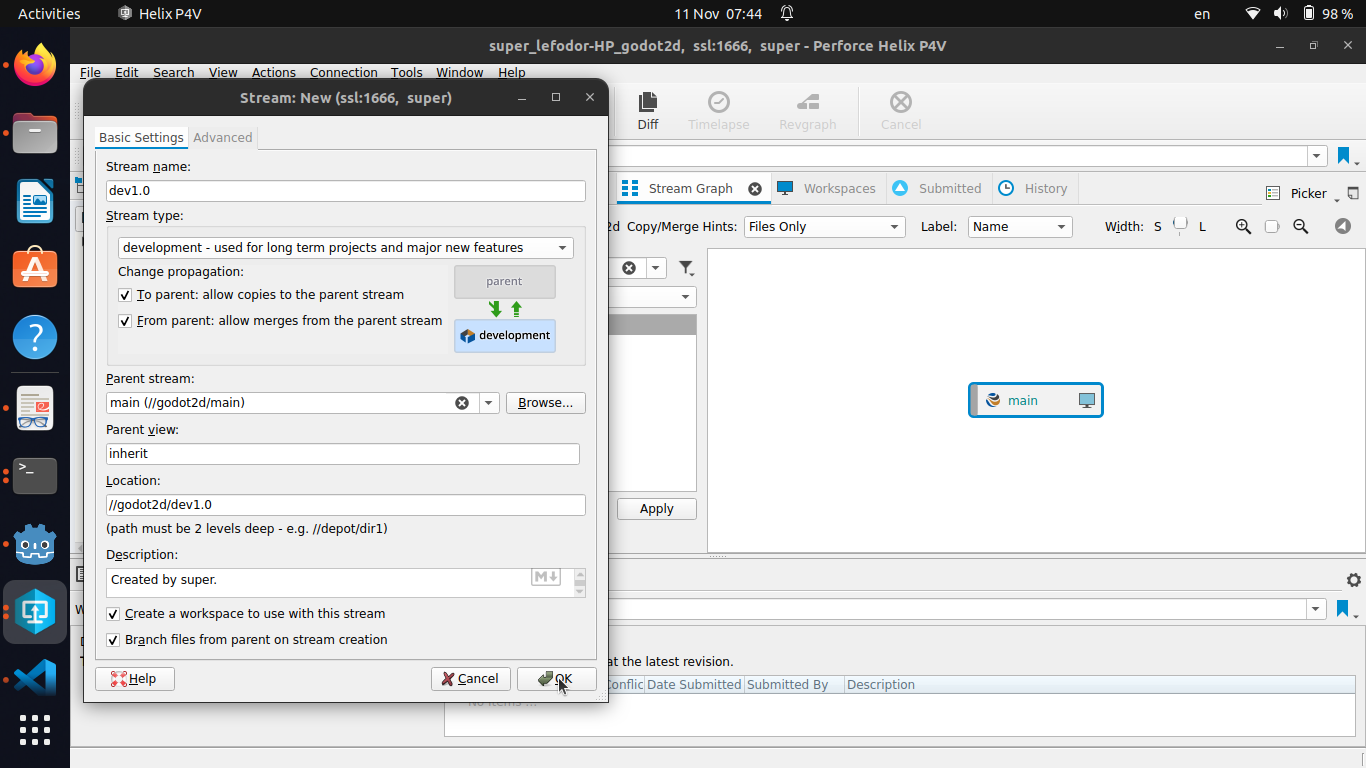
\includegraphics[width=\textwidth]{new-stream-for-branching.png}
      \caption{p4v new stream for branching}
      \label{fig:new-stream-for-branching}
\end{figure}
A new development stream (branch) has been created:
\begin{figure}[H]
    \centering
    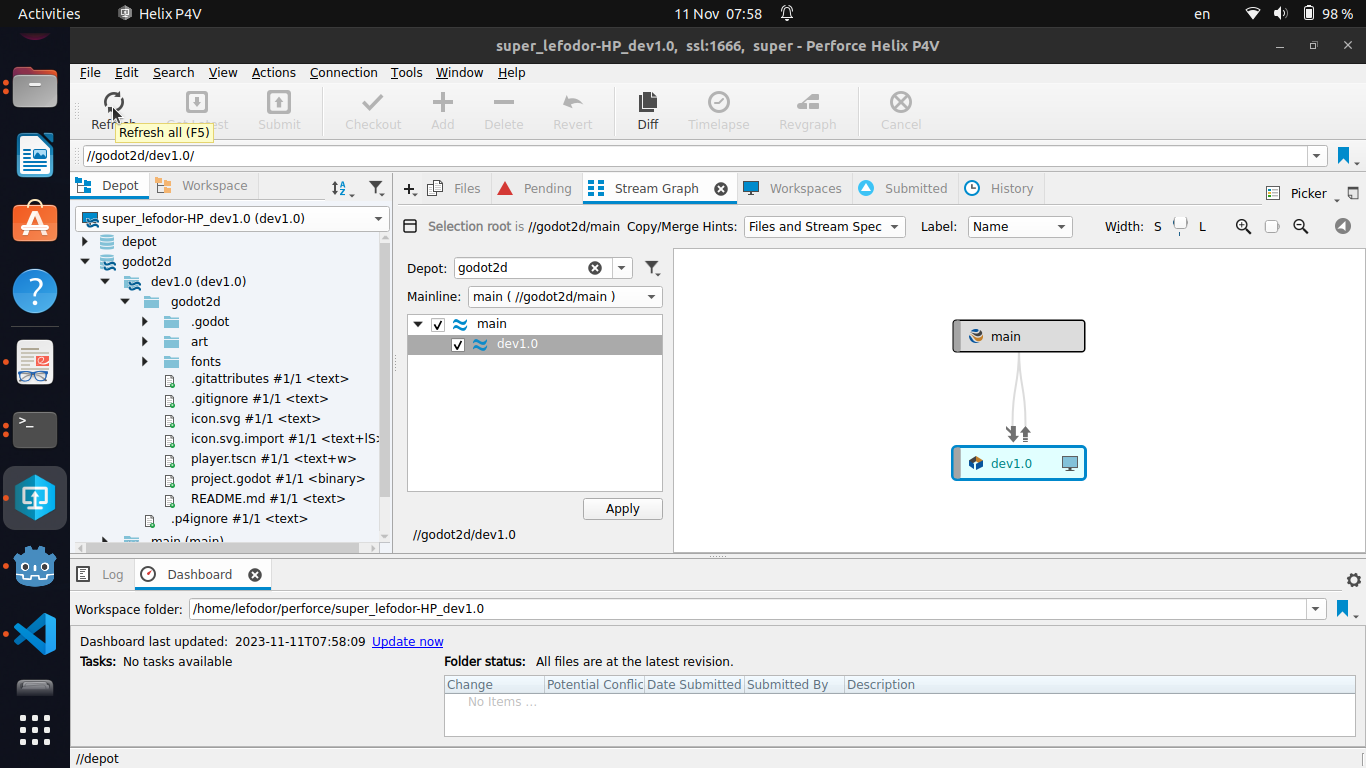
\includegraphics[width=\textwidth]{new-branch-dev1.0.png}
      \caption{new stream (branch) dev1.0}
      \label{fig:new-branch-dev1.0}
\end{figure}
From this point onwards, all changes are to be made on the development stream and later merged back to the more stable
main stream.

\subsection{Development steps cont'd}
\begin{enumerate}[resume]
    \item Coding player scene.
\end{enumerate}